%=======================02-713 LaTeX template, following the 15-210 template==================
%
% You don't need to use LaTeX or this template, but you must turn your homework in as
% a typeset PDF somehow.
%
% How to use:
%    1. Update your information in section "A" below
%    2. Write your answers in section "B" below. Precede answers for all 
%       parts of a question with the command "\question{n}{desc}" where n is
%       the question number and "desc" is a short, one-line description of 
%       the problem. There is no need to restate the problem.
%    3. If a question has multiple parts, precede the answer to part x with the
%       command "\part{x}".
%    4. If a problem asks you to design an algorithm, use the commands
%       \algorithm, \correctness, \runtime to precede your discussion of the 
%       description of the algorithm, its correctness, and its running time, respectively.
%    5. You can include graphics by using the command \includegraphics{FILENAME}
%
\documentclass[11pt]{article}
\usepackage{amsmath,amssymb,amsthm}
\usepackage{graphicx}
\usepackage[margin=1in]{geometry}
\usepackage{fancyhdr}
\usepackage[table,xcdraw]{xcolor}
\setlength{\parindent}{0pt}
\setlength{\parskip}{5pt plus 1pt}
\setlength{\headheight}{13.6pt}
\newcommand\question[2]{\vspace{.25in}\hrule\textbf{#1 #2}\vspace{.5em}\hrule\vspace{.10in}}
\renewcommand\part[1]{\vspace{.10in}\textbf{(#1)}}
\newcommand\algorithm{\vspace{.10in}\textbf{Algorithm: }}
\newcommand\correctness{\vspace{.10in}\textbf{Correctness: }}
\newcommand\runtime{\vspace{.10in}\textbf{Running time: }}
\pagestyle{fancyplain}
\lhead{\textbf{\NAME}}
\chead{\textbf{HW\HWNUM}}
\rhead{605.202.81, \today}

\begin{document}\raggedright
%Section A==============Change the values below to match your information==================
\newcommand\NAME{Sean Connor}  % your name
\newcommand\HWNUM{1}              % the homework number
%Section B==============Put your answers to the questions below here=======================

% no need to restate the problem --- the graders know which problem is which,
% but replacing "The First Problem" with a short phrase will help you remember
% which problem this is when you read over your homeworks to study.

\question{Q1}{} 

The primary reason that binary is used - and not ternary - is because computers are based on transistor technology. Transistors, in general, are switches that provide an "on" state and an "off" state. Because of this, it would be much more complex and difficult to implement as a ternary system.

\begin{table}[h!]
	\begin{center}
		\begin{tabular}{r|r|r} % <-- Alignments: 1st column left, 2nd middle and 3rd right, with vertical lines in between
			\textbf{Decimal} & \textbf{Binary} & \textbf{Ternary}\\
			\hline
			0 & 0000 & 0000\\
			1 & 0001 & 0001\\
			2 & 0010 & 0002\\
			3 & 0011 & 0010\\
			4 & 0100 & 0011\\
			5 & 0101 & 0012\\
			6 & 0110 & 0020\\
			7 & 0111 & 0021\\
			8 & 1000 & 0022\\
			9 & 1001 & 0100\\
			10 & 1010 & 0101\\
			11 & 1011 & 0102\\
			12 & 1100 & 0110\\
			13 & 1101 & 0111\\
			14 & 1110 & 0112\\
			15 & 1111 & 0120\\
		\end{tabular}
	\end{center}
\end{table}


\question{Q2}{}
Assuming index starts at 0 (as opposed to 1). Because the order is row major order, the calculations are as follows:

\[RM[i][j] = 100 + i(20)(4) + j(4) = 100 + 80i + 4j\] 

\[RM[5][3] = 100 + 5(80) + 3(4) = 512\] 

\[RM[9][19] = 100 + 9(80) + 19(4) = 896\] 


\question{Q3}{}
\part{a}
The maximum number of non-zero elements is one half of the NxN square matrix, inclusive of the diagonal. This is given by:

\[\frac{N \cdot N}{2} + N\]

This can be simplified to:

\[\frac{N^2 - N}{2} + \frac{2N}{2} = \frac{N^2 + N}{2} = \frac{N(N+1)}{2} \]

\part{b}
The numbers can be stored sequentially by using arrays of the following form:
% Please add the following required packages to your document preamble:
% \usepackage[table,xcdraw]{xcolor}
% If you use beamer only pass "xcolor=table" option, i.e. \documentclass[xcolor=table]{beamer}
\begin{table}[!htbp]
	\centering
	\begin{tabular}{
			>{\columncolor[HTML]{FFFE65}}l lllllllllllllll}
		\textbf{i}                     & 0 & 1 & 1 & 2 & 2 & 2 & 3 & 3 & 3 & 3 & 4  & 4  & 4  & 4  & 4  \\
		\textbf{j}                     & 0 & 0 & 1 & 0 & 1 & 2 & 0 & 1 & 2 & 3 & 0  & 1  & 2  & 3  & 4  \\
		\textbf{k}                     & 0 & 1 & 2 & 3 & 4 & 5 & 6 & 7 & 8 & 9 & 10 & 11 & 12 & 13 & 14 \\
		\textbf{delta} & 0 & 0 & 0 & 1 & 1 & 1 & 3 & 3 & 3 & 3 & 6  & 6  & 6  & 6  & 6 
	\end{tabular}
\end{table}

\part{c}
First, see the the following holds true:

\[k=i+j+\Delta_(i-1)\]

In addition, observe that for each increment of i, the delta value increases according the triangular number series.

Thus, k can be represented by the following:

\[k = \Delta_i + j = \frac{i^2 + i}{2} + j \]


\question{Q4}{}
\part{a}
The equation can be given by the following:

\[N + 2(N-1) = N + 2N - 2 = 3N -2 \]

\part{b}
The numbers can be stored sequentially by using arrays of the following form:

\begin{table}[!htbp]
	\centering
	\begin{tabular}{
			>{\columncolor[HTML]{FFFE65}}l llllllllllllll}
		\textbf{i}                     & 0 & 0 & 1 & 1 & 1 & 2 & 2 & 2 & 3 & 3 & 3  & 4  & 4  & 4  \\
		\textbf{j}                     & 0 & 1 & 0 & 1 & 2 & 1 & 2 & 3 & 2 & 3 & 4  & 3  & 4  & 5  \\
		\textbf{k}                     & 0 & 1 & 2 & 3 & 4 & 5 & 6 & 7 & 8 & 9 & 10 & 11 & 12 & 13 
	\end{tabular}
\end{table}

\part{c}
k can be represented by the following:

\[k = 2i + j \]


\question{Q5}{}
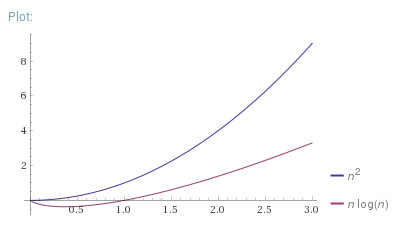
\includegraphics[]{pic1.jpg}
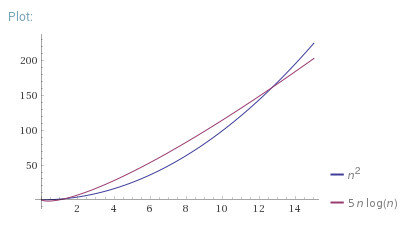
\includegraphics[]{pic2.jpg}
\newline

The case of n\textsuperscript{2} will generally quickly outpace nlg(n). We can try to solve for n via the following:

\[an^2 = bnlg(n)\]
\[\frac{a}{b}=\frac{1}{n}lg(n)\]
\[\frac{a}{b}=lg(n^\frac{1}{n})\]
\[e^\frac{a}{b} = n^\frac{1}{n}\]

\question{Q6}{}
\[1 hr = 3600 s = 3.6e9\mu s\]
\[lg(n) = 3.6e9\mu s\]
\[n = e^{3.6e9}\]

\question{Q7}{}
\[1 hr = 3600 s = 3.6e9\mu s\]
\[n^3 = 3.6e9\mu s\]
\[n = (3.6e9)^{\frac{1}{3}}\]



\end{document}
